\documentclass{article}

\usepackage[utf8]{inputenc}
\usepackage{enumerate}
\usepackage{graphicx}

\begin{document}
\begin{enumerate}[1)]
    \item{ % 1)
        Primero hacemos el desarrollo en serie de Taylor de los puntos que queremos utilizar:

        \[ u_{i-3} = u_i - 3 h u_i' + \frac{9}{2} h^2 u_i'' - \frac{27}{6} h^3 u_i''' \
                     + \frac{81}{24} h^4 u_i^{(4)} + O(h^5) \]

        \[ u_{i-2} = u_i - 2 h u_i' + \frac{4}{2} h^2 u_i'' - \frac{8}{6} h^3 u_i''' \
                     + \frac{16}{24} h^4 u_i^{(4)} + O(h^5) \]

        \[ u_{i-1} = u_i - h u_i' + \frac{1}{2} h^2 u_i'' - \frac{1}{6} h^3 u_i''' \
                     + \frac{1}{24} h^4 u_i^{(4)} + O(h^5) \]

        \[ u_{i+1} = u_i + h u_i' + \frac{1}{2} h^2 u_i'' + \frac{1}{6} h^3 u_i''' \
                     + \frac{1}{24} h^4 u_i^{(4)} + O(h^5) \]

        Queremos aproximar la segunda derivada mediante la fórmula dada. Si expandemos ésta obtenemos:

        \begin{eqnarray*}
            a u_{i-3} + b u_{i-2} + c u_{i-1} + d u_i + e u_{i+1} = &&(a+b+c+d+e) u_i + h (-3a -2b -c + e) u_i' \\
                                &+& \frac{h^2}{2} (9a + 4b + c + e) u_i'' + \frac{h^3}{6} (-27a -8b-c+e) u_i''' \\ 
                                &+& \frac{h^4}{24} (81a+16b+c+e) u_i^{(4)} + O(h^5)
        \end{eqnarray*}

        Si igualamos este resultado a $\frac{h^2}{2} u_i'' + O(h^5)$ obtenemos el siguiente sistema de ecuaciones
        algebraicas:

        \[ \left( 
            \begin{array}{rrrrr} 
                1 &  1 &  1 & 1 & 1 \\
               -3 & -2 & -1 & 0 & 1 \\
                9 &  4 &  1 & 0 & 1 \\
              -27 & -8 & -1 & 0 & 1 \\
               81 & 16 &  1 & 0 & 1 \\
            \end{array}
           \right)
           \left(
            \begin{array}{c}
                a \\
                b \\
                c \\
                d \\
                e \\
            \end{array}
           \right)
           =
           \left(
            \begin{array}{c}
                0 \\
                0 \\
                1 \\
                0 \\
                0 \\
            \end{array}
           \right)
        \]

        La solución de este sistema es:

        \[
           \left(
            \begin{array}{c}
                a \\
                b \\
                c \\
                d \\
                e \\
            \end{array}
           \right)
           =
           \left(
            \begin{array}{c}
                -\frac{1}{24} \\
                 \frac{1}{6} \\
                 \frac{1}{4} \\
                -\frac{5}{6} \\
                 \frac{11}{24} \\
            \end{array}
           \right)
        \]

        Reemplazando obtenemos:

        \[ -\frac{1}{24} u_{i-3} + \frac{1}{6} u_{i-2} + \frac{1}{4} u_{i-1} - \frac{5}{6} u_i + \frac{11}{24} u_{i+1} = 
        \frac{h^2}{2}u_i'' + O(h^5) \]

        Que puede reescribirse como:

        \[ \frac{-u_{i-3} + 4 u_{i-2} + 6 u_{i-1} -20 u_i + 11 u_{i+1}}{12 h^2} = u_i'' + O(h^3) \]
    }
    \item{ % 2)
        El problema de conducción de calor en 1D se expresa como:

        \[ \frac{\partial T}{\partial t} + k \Delta T + c (T - T_{amb}) + Q = 0 \qquad 0 < x < L \]

        El término $\frac{\partial T}{\partial t}$ se anula al tratarse del caso estacionario. Considerando
        esto y los valores dados para las constantes, el problema puede reescribirse como:

        \[ \frac{\partial^2 T}{\partial x^2} + T = 4 \left(x - \frac{1}{2} \right)^2 - 1 \qquad 0 < x < 1 \]

        Utilizando el método de diferencias finitas y haciendo las siguientes aproximaciones:

        \[ \left( \frac{\partial^2 T}{\partial x^2} \right)_i 
           \approx
           \frac{T_{i+1} - 2 T_i + T_{i-1}}{h^2} \]

        \[ \left( \frac{\partial T}{\partial x} \right)_i 
           \approx
           \frac{T_{i+1} - T_{i-1}}{2 h}, \]

        donde $h$ es el paso de la malla (uniforme) utilizada, se obtienen los siguientes resultados
        para distintos $N$ (cantidad de segmentos en la malla: $N = \frac{1}{h}$):

        \begin{tabular}{|c|c|c|}
            \hline
            \textbf{N} & \textbf{Error} & \textbf{Proporción mejora} \\
            \hline
             2 & 0.0105 & \\
            \hline
             4 & 0.0022 & 4.6903 \\
            \hline
             8 & 5.1638e-04 & 4.3316 \\
            \hline
            16 & 1.2390e-04 & 4.1678 \\
            \hline
            32 & 3.0328e-05 & 4.0852 \\
            \hline
            64 & 7.5012e-06 & 4.0431 \\
            \hline
            128 & 1.8652e-06 & 4.0217 \\
            \hline
            256 & 4.6503e-07 & 4.0109 \\
            \hline
            512 & 1.1610e-07 & 4.0054 \\
            \hline
            1024 & 2.9007e-08 & 4.0025 \\
            \hline
            2048 & 7.2540e-09 & 3.9988 \\
            \hline
        \end{tabular}

        El error se obtuvo dividiendo la norma euclídea de la diferencia entre la aproximación y
        la solución exacta por la norma euclídea de la solución exacta:

        \[ \mbox{error} = \frac{\left|\left| x_{aprox} - x_{exacta}\right|\right|_2}{\left|\left| x_{exacta} \right|\right|_2} \]

        En la tabla puede apreciarse cómo la solución es aproximadamente cuatro veces mejor cuando
        se duplica el número de intervalos. \textit{(Supongo que el hecho de que esta proporción vaya 
        disminuyendo se debe a que a mayor número de intervalos hay mayor error numérico.)}

        Para el caso $N = 8$, la gráfica del resultado es:

        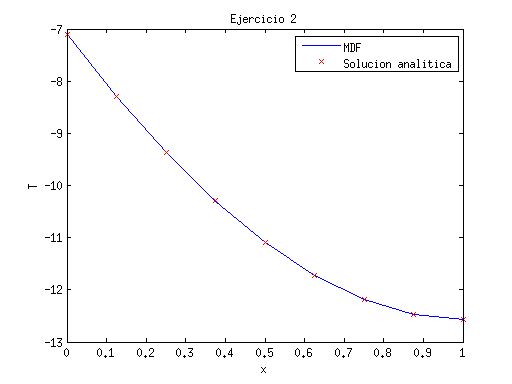
\includegraphics[width=\textwidth]{ej2_N_8.png}
    }
    \item{ % 3)
        \begin{enumerate}[a)]
            \item{ % a)
                Utilizando diferencias finitas y las aproximaciones:

                \[ \left( \frac{\partial^2 \phi}{\partial x^2} \right)_{l, m}
                   \approx
                   \frac{\phi_{l-1,m} - 2 \phi_{l,m} + \phi_{l+1,m}}{dx^2} \]

                \[ \left( \frac{\partial^2 \phi}{\partial y^2} \right)_{l, m}
                   \approx
                   \frac{\phi_{l,m-1} - 2 \phi_{l,m} + \phi_{l,m+1}}{dx^2} \]

                se obtiene la siguiente solución:

                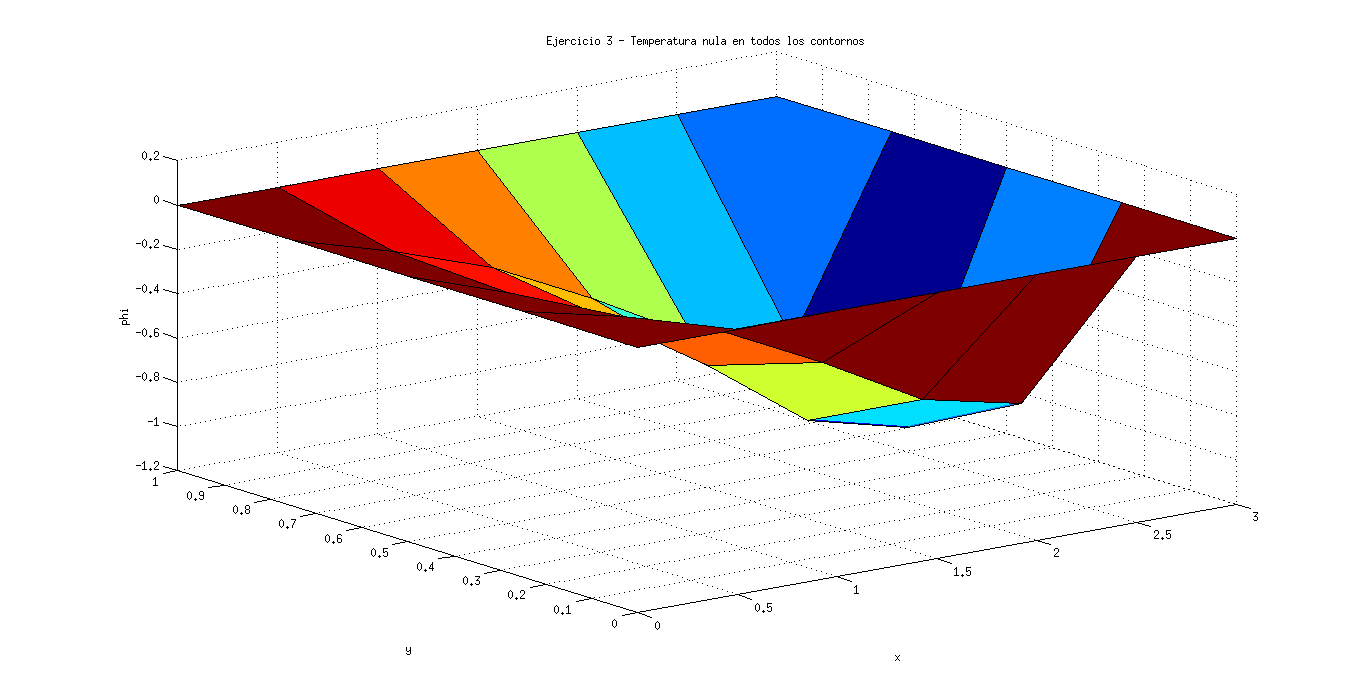
\includegraphics[width=\textwidth]{ej3_Dirichlet_0.png}
            }
            \item{ % b)
                El inciso anterior correspondía al caso en que se impone una temperatura
                nula en todos los bordes. Si en cambio se impone una temperatura 
                $\bar{T} = 100$ se obtiene:

                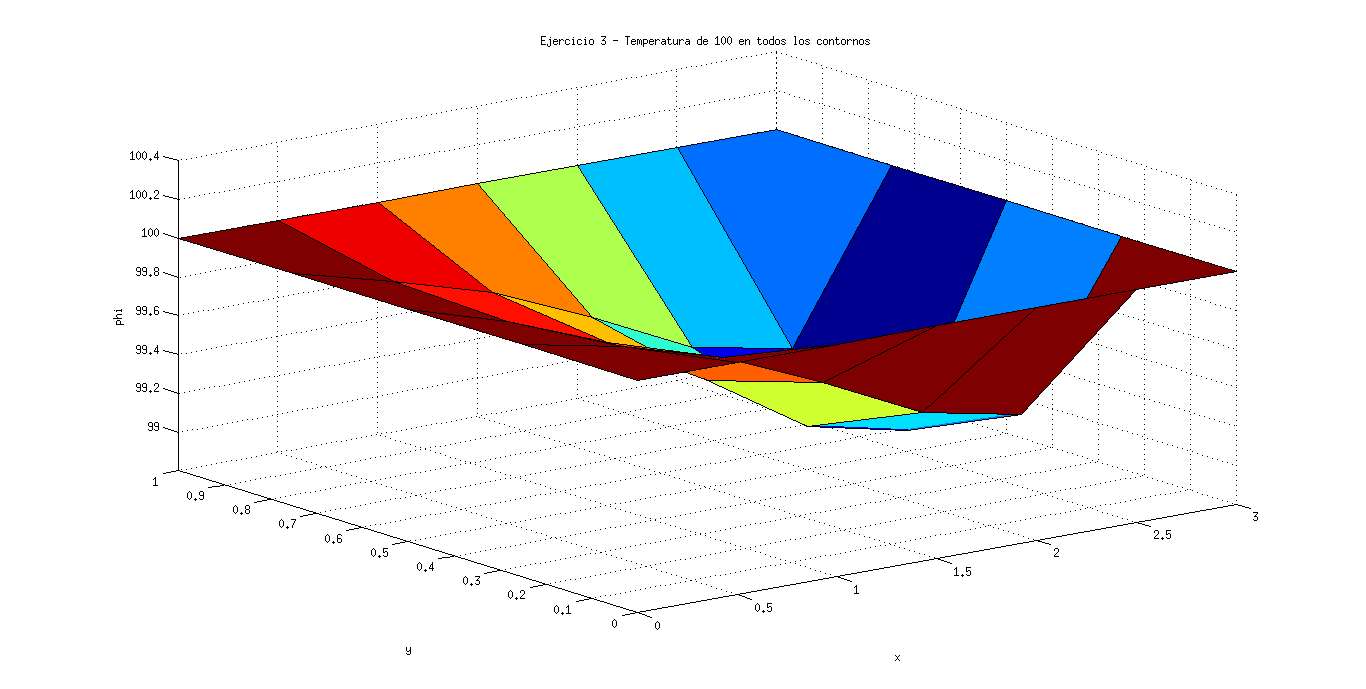
\includegraphics[width=\textwidth]{ej3_Dirichlet_100.png}

                Puede apreciarse que la solución tiene la misma forma que en el inciso
                anterior, excepto porque toda la superficie está aumentada en $100$
                en el eje $\phi$.

                Se pueden combinar los problemas imponiendo, por ejemplo, una temperatura
                de $100$ en el borde inferior y en el izquierdo y una temperatura nula
                en el borde superior y en el derecho:

                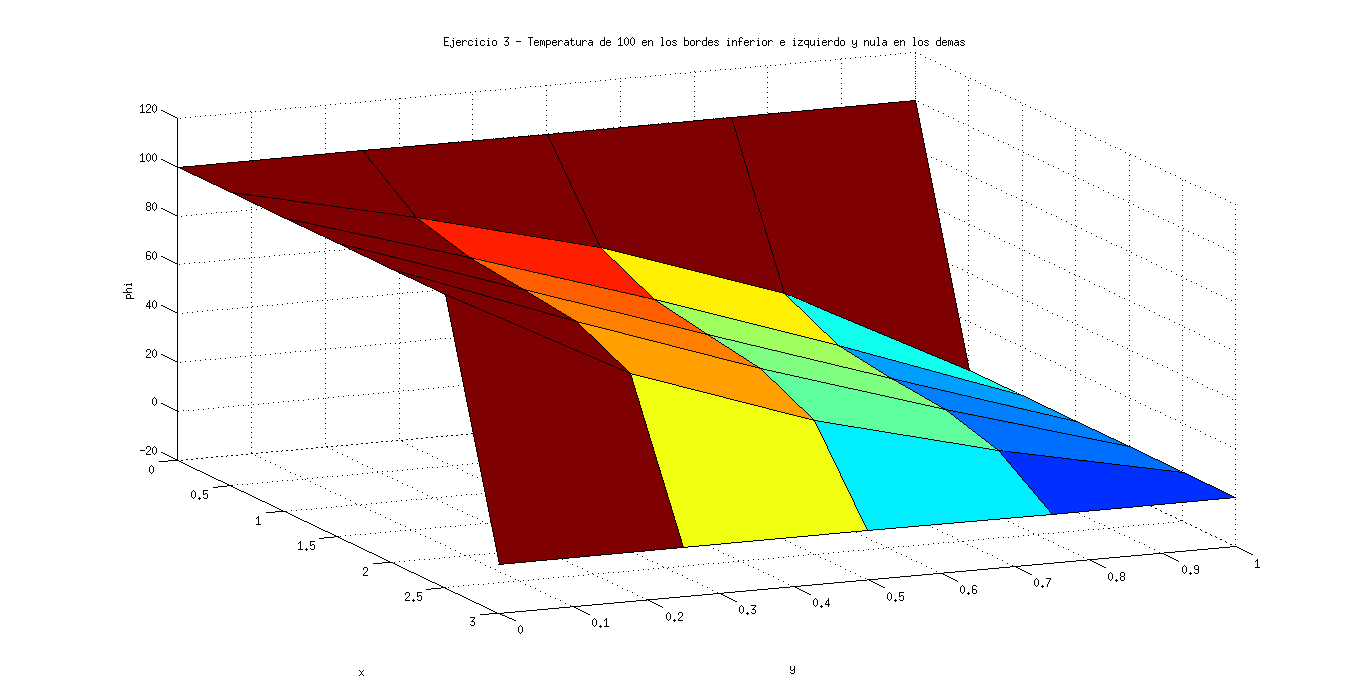
\includegraphics[width=\textwidth]{ej3_Dirichlet_0_y_100.png}

                En este caso puede apreciarse claramente que en las esquinas una de las
                condiciones tiene prioridad. Si esto es un problema, una posible solución
                es promediar ambas condiciones (si son del mismo tipo). Haciendo esto
                el resultado obtenido es:

                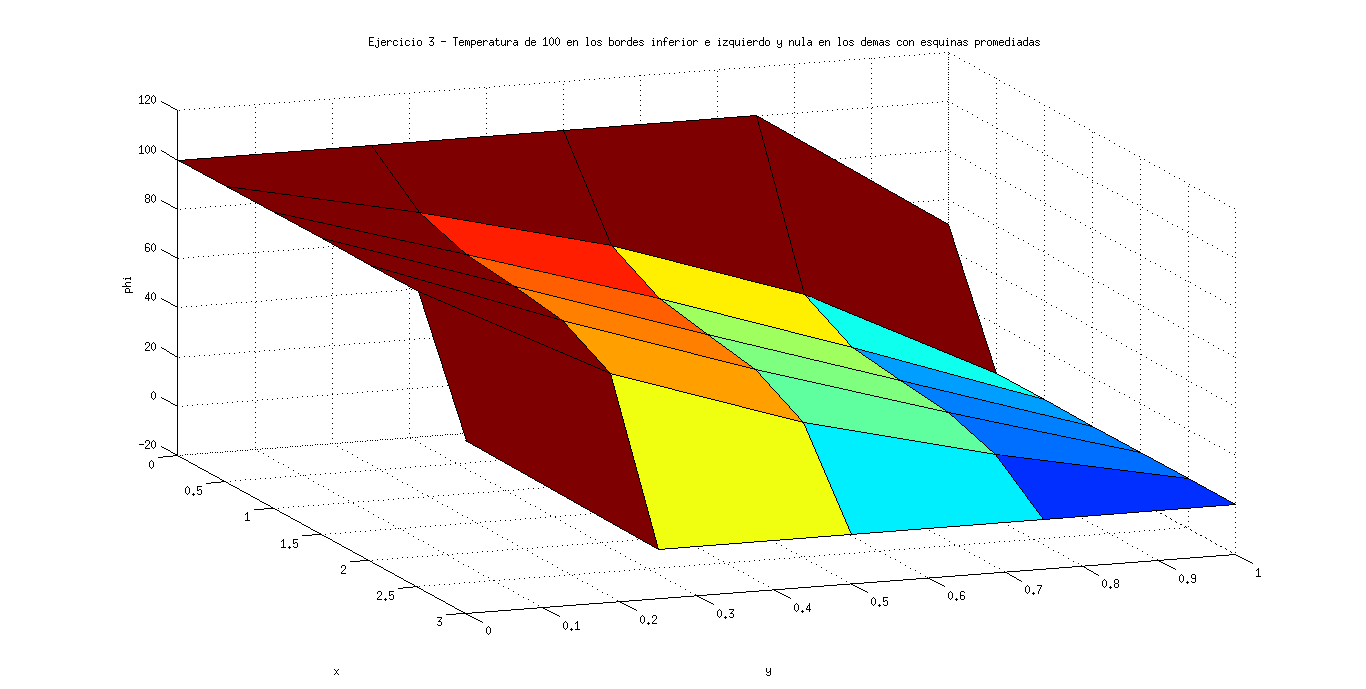
\includegraphics[width=\textwidth]{ej3_Dirichlet_0_y_100_esquinas_promediadas.png}
            }
            \item{ % c)
                Para tratar con las condiciones de flujo se utilizaron las siguientes aproximaciones:

                \[ \left( \frac{\partial \phi}{\partial x} \right)_{l,m} 
                   \approx
                   \frac{3 \phi_{l,m} - 4 \phi_{l-1,m} + \phi_{l-2,m}}{2 dx} \]

                \[ \left( \frac{\partial \phi}{\partial x} \right)_{l,m} 
                   \approx
                   \frac{-3 \phi_{l,m} + 4 \phi_{l+1,m} - \phi_{l+2,m}}{2 dx} \]

                (Aproximaciones análogas se usan para 
                $\frac{\partial \phi}{\partial y}$).

                El uso de una u otra aproximación depende de si se necesita usar puntos que están
                "adelante" o "atrás" del punto donde se está evaluando la derivada.

                Si ahora se impone una temperatura de $100$ en los bordes superior, izquierdo y
                derecho y un flujo de calor nulo en el contorno inferior, el resultado es:

                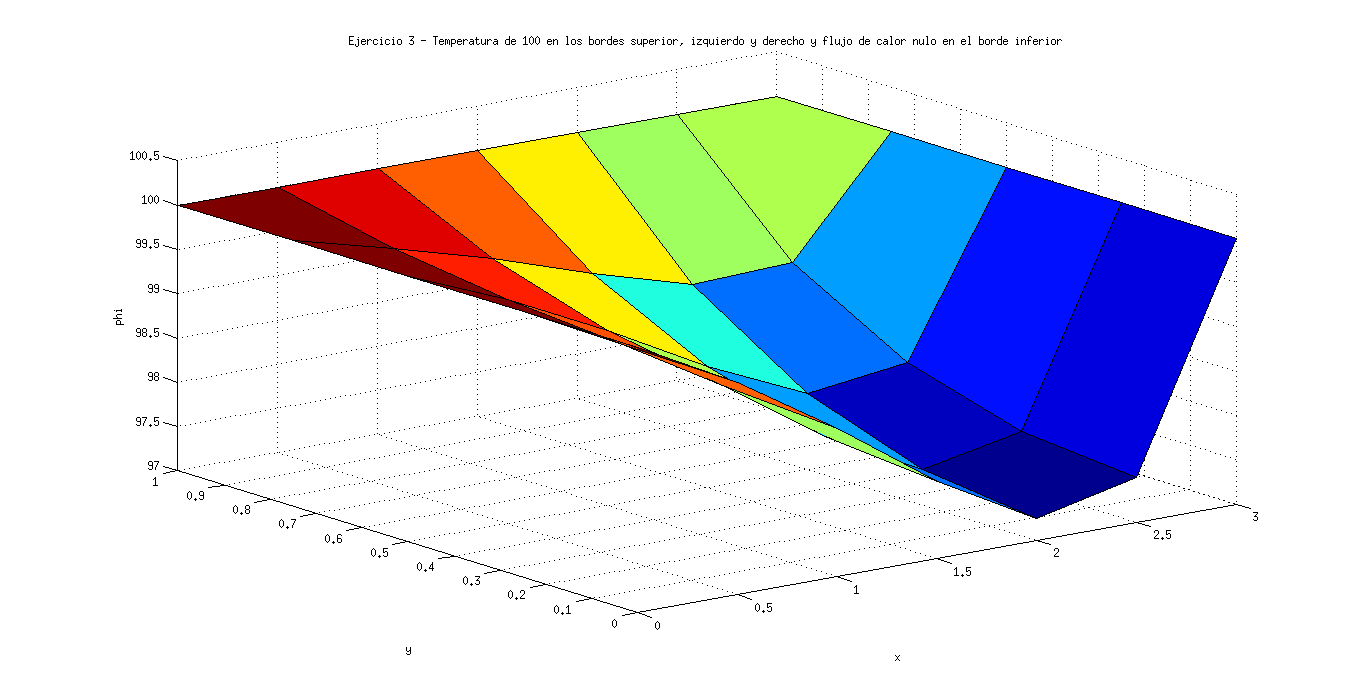
\includegraphics[width=\textwidth]{ej3_Neumann_0_Dirichlet_100.png}

                Para este problema, utilizar sólo condiciones de tipo Neumann causa una
                indeterminación que, en el método, se traduce en una matriz singular
                (no invertible). Si se usan sólo condiciones de flujo nulo pero se
                fija la temperatura para un punto que no esté en una esquina, entonces se puede
                obtener un resultado. Fijando la temperatura del punto $(0.5; 0.25)$ en $100$
                el resultado es:

                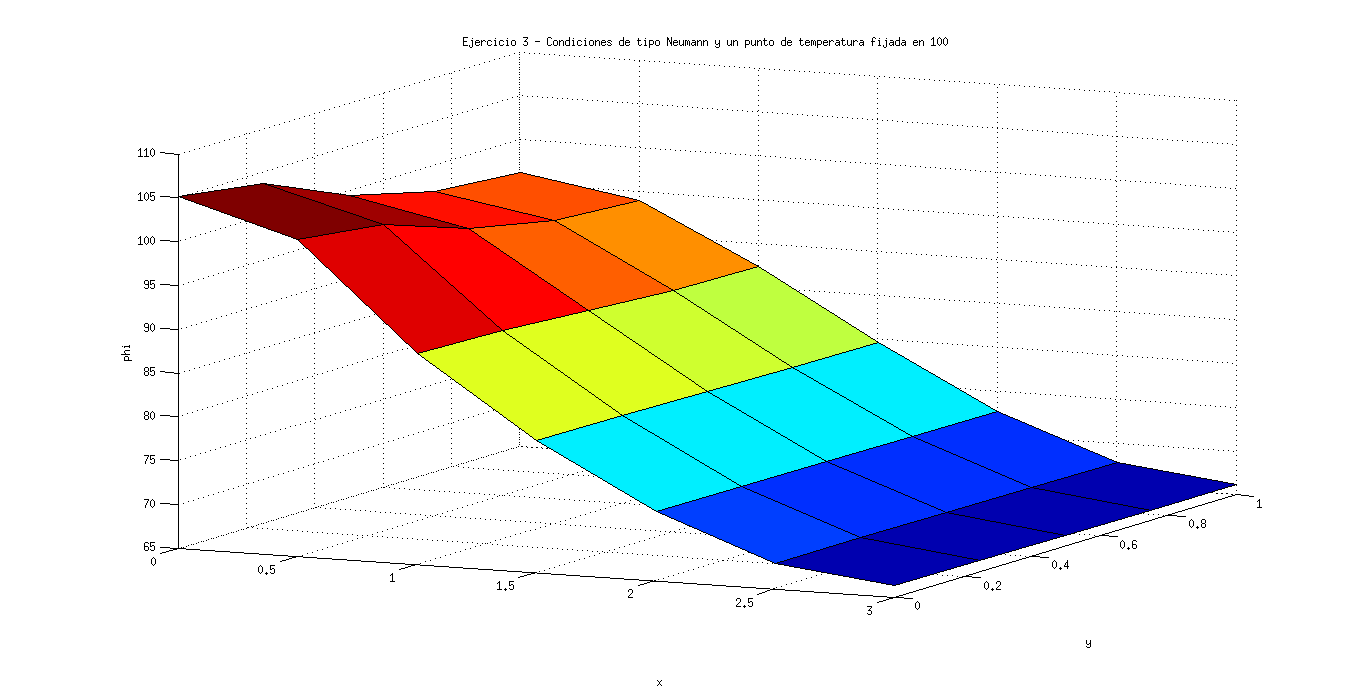
\includegraphics[width=\textwidth]{ej3_Neumann_0_Punto_fijado_100.png}

                \textit{(Si se fija la temperatura de un punto que esté en una esquina, se sigue
                obteniendo una matriz singular, no sé por qué.)}
            }
        \end{enumerate}
    }
    \item{ % 4)
        Como se trata de una malla no uniforme, necesitamos aproximar las derivadas de otra manera.
        Si se quiere obtener la derivada primera para el punto $x_i$, cuyos puntos vecinos
        a izquierda y derecha están a una distancia de $h_-$ y $h_+$, respectivamente, se plantea
        primero el desarrollo en serie de Taylor de los puntos vecinos:

        \[ \phi_{i+1} = \phi_i + h_+ \phi_i' + O(h_+^2) \]
        \[ \phi_{i-1} = \phi_i - h_- \phi_i' + O(h_-^2) \]

        Y despejando la derivada:

        \[ \phi_i' \approx \frac{\phi_{i-1} + \phi_{i+1}}{h_- + h_+} \]

        Haciendo algo análogo para la segunda derivada se obtiene:

        \[ \phi_i'' \approx \frac{2}{h_+(h_+ + h_-)} \phi_{i+1} - \frac{2}{h_-h_+} \phi_i 
                      + \frac{2}{h_-(h_++h_-)} \phi_{i-1} \]

        El resultado de aplicar estas aproximaciones puede apreciarse en la siguiente gráfica:

        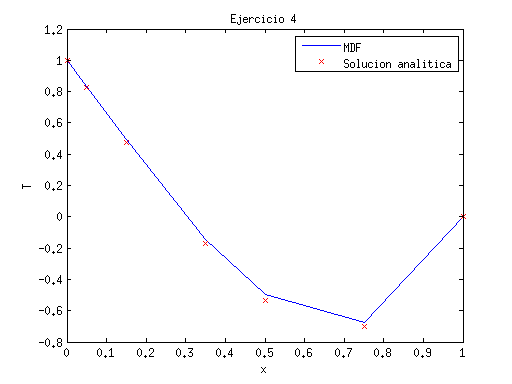
\includegraphics[width=\textwidth]{ej4.png}

        Utilizando mallas con menores separaciones, pero manteniendo la relación de distancias
        (interpolación lineal), se obtienen los siguientes resultados:

        \begin{tabular}{|c|c|c|}
            \hline
            \textbf{N} & \textbf{Error} & \textbf{Proporción mejora} \\
            \hline
            7 & 0.0365 & \\
            \hline
            13 & 0.0094 & 3.8766 \\
            \hline
            25 & 0.0024 & 3.9098 \\
            \hline
            49 & 6.1014e-04 & 3.9484 \\
            \hline
            97 & 1.5358e-04 & 3.9726 \\
            \hline
            193 & 3.8532e-05 & 3.9859 \\
            \hline
            385 & 9.6502e-06 & 3.9929 \\
            \hline
            769 & 2.4147e-06 & 3.9964 \\
            \hline
            1537 & 6.0395e-07 & 3.9982 \\
            \hline
            3073 & 1.5100e-07 & 3.9995 \\
            \hline
        \end{tabular}

        Nuevamente, al (casi) duplicarse el número de nodos, el error disminuye casi cuatro
        veces. Sin embargo, a diferencia del ejercicio 2, la proporción de mejora aumenta
        al aumentar el número de nodos.
    }
    \item{ % 5)
        En los videos adjuntos \texttt{explicito.avi}, \texttt{implicito.avi} y \texttt{cn.avi}
        se pueden ver los resultados de resolver este problema con los métodos de forward
        Euler, backward Euler y Crank-Nicholson, respectivamente. Se obtuvo el primer segundo
        y se usó $\Delta t = 0.01$.

        Los resultados son casi indistinguibles, pero al hacerlos se apreciaron algunas
        diferencias importantes entre los métodos.
        
        El método de forward Euler no converge para cualquier paso de tiempo (ya con 
        $\Delta t = 0.05$ hay divergencia). El de backward Euler llega al mismo resultado
        independientemente del paso del tiempo. El método de Crank-Nicholson, si bien
        llega al resultado para pasos de tiempo con los que el de forward Euler no lo hace,
        no parece admitir pasos de tiempo arbitrariamente grandes. Para, por ejemplo,
        un paso de $\Delta t = 1$, y simulando los primeros cincuenta segundos, el resultado
        alterna entre la solución correcta y una muy distinta.

        En cuanto al tiempo, el primero demora $0.99$ segundos, el segundo $3.48$ y el
        tercero $3.54$ (y, aunque no es necesario, se implementó el método de forward
        Euler con una inversión de matriz al igual que los otros, así que es de esperar
        que sea significativamente mayor la diferencia de tiempos entre éste y los
        otros dos métodos si se lo implementa sin usar una matriz).
    }
\end{enumerate}
\end{document}
